\documentclass[]{article}
\usepackage{lmodern}
\usepackage{amssymb,amsmath}
\usepackage{ifxetex,ifluatex}
\usepackage{fixltx2e} % provides \textsubscript
\ifnum 0\ifxetex 1\fi\ifluatex 1\fi=0 % if pdftex
  \usepackage[T1]{fontenc}
  \usepackage[utf8]{inputenc}
\else % if luatex or xelatex
  \ifxetex
    \usepackage{mathspec}
    \usepackage{xltxtra,xunicode}
  \else
    \usepackage{fontspec}
  \fi
  \defaultfontfeatures{Mapping=tex-text,Scale=MatchLowercase}
  \newcommand{\euro}{€}
\fi
% use upquote if available, for straight quotes in verbatim environments
\IfFileExists{upquote.sty}{\usepackage{upquote}}{}
% use microtype if available
\IfFileExists{microtype.sty}{%
\usepackage{microtype}
\UseMicrotypeSet[protrusion]{basicmath} % disable protrusion for tt fonts
}{}
\ifxetex
  \usepackage[setpagesize=false, % page size defined by xetex
              unicode=false, % unicode breaks when used with xetex
              xetex]{hyperref}
\else
  \usepackage[unicode=true]{hyperref}
\fi
\hypersetup{breaklinks=true,
            bookmarks=true,
            pdfauthor={Wantee Wang},
            pdftitle={Knowledge Embedding},
            colorlinks=true,
            citecolor=blue,
            urlcolor=blue,
            linkcolor=magenta,
            pdfborder={0 0 0}}
\urlstyle{same}  % don't use monospace font for urls
\setlength{\parindent}{0pt}
\setlength{\parskip}{6pt plus 2pt minus 1pt}
\setlength{\emergencystretch}{3em}  % prevent overfull lines
\setcounter{secnumdepth}{0}

\title{Knowledge Embedding}
\author{Wantee Wang}
\date{2015-03-24 10:05:58 +0800}
\usepackage[sort&compress, numbers]{natbib}

\begin{document}
\maketitle

Neural Networks are applied in many fields of Machine Learning. Due to
their natural property, it is suitable to use them to estimate the
\emph{distribution representations} from some knowledge source. This
kind of representation may be referred as \emph{knowledge embedding}.

\href{http://en.wikipedia.org/wiki/Embedding}{Embedding},
mathematically, denotes one instance of some mathematical structure
contained within another instance. In Machine Learning context, it often
means to transfer a sparse coding of an instance to a more dense coding,
e.g., a 1-of-V coding to a low dimension vector.

\section{Word2Vec}\label{word2vec}

The first successful application of NN-based embedding is
\href{https://code.google.com/p/word2vec/}{word2vec}, which converts a
word to a continuous vector.

The inspiration \cite{mikolov2013efficient} of word2vec is from the
observation that neutral network language model can be successfully
trained in two steps: first, continuous word vectors are learned using
simple model, and then the N-gram NNLM is trained on top of these
distributed representations of words. Then the authors spend lots of
work on learning word vectors. Thus the word-to-vector procedure can be
seen as a feature extraction step for language modelling.

To show the innovation of word2vec, we first consider the traditional
N-gram NNLM. The architecture of NNLM \cite{bengio2003neural} is shown
in following figure (\autoref{fig:nnlm})

\begin{figure}[h]\centering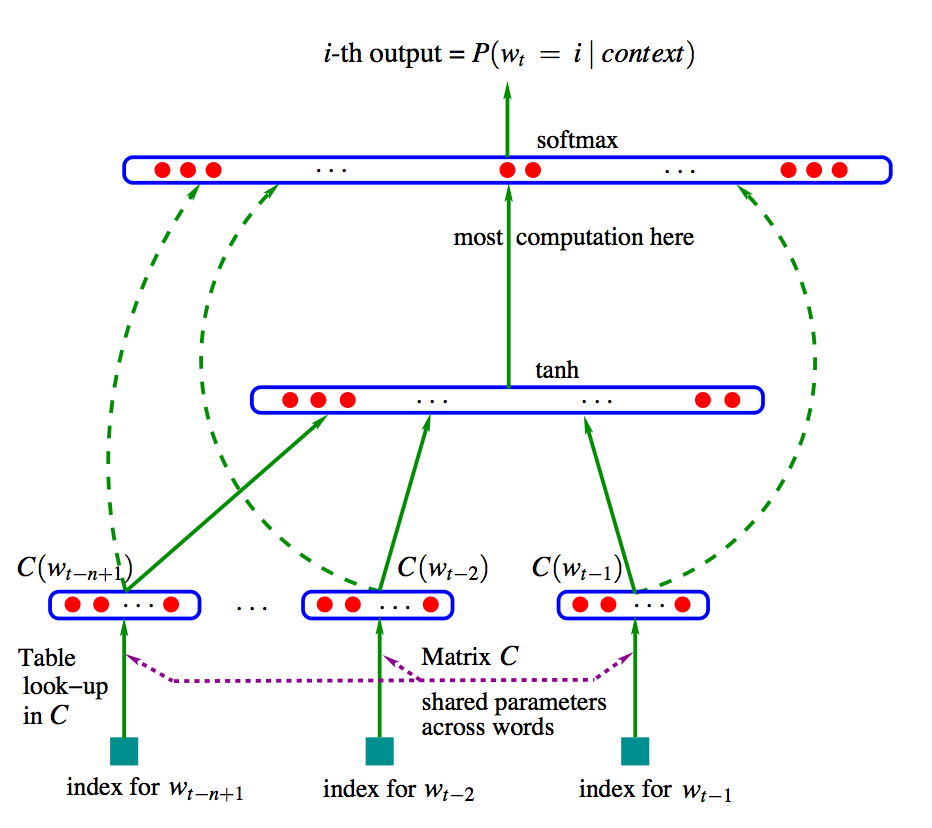
\includegraphics[width=\textwidth]{source//images/posts/nnlm.png}\caption{Architecture of NNLM}\label{fig:nnlm}\end{figure}

The NNLM consists of input, projection, hidden and output layers. At the
input layer, \(N\) previous words are encoded using 1-of-V coding, where
\(V\) is size of the vocabulary. The input layer is then projected to a
projection layer that has dimensionality \(N \times D\). Next,
projection layer is connected to the hidden layer, whose size is \(H\),
finally, we reach the output layer, which is of size \(V\), through
hidden layer.

Therefore, the computational complexity per each training example is

\[
Q = N \times D + N \times D \times H + H \times V
\]

Where the domination term is \(H \times V\). However several output
layer optimisations method can avoid it, such as \emph{Hierarchical
Softmax} which reduce the output term to \(H \times \log_2(V)\). Then
the domination term becomes \(N \times D \times H\).

It is can be seen from above discussion the most complexity is caused by
the non-linear hidden layer in the model(if we check out the RNN LM
model, same conclusion can be derived, i.e., the hidden layer occupied
most computational resources).

However, if the goal is only to extract word embeddings, we can
sacrifice some precision of NN models. This leads to the key point of
speedup of word2vec, that is by \textbf{removing the non-linear hidden
layer}, and used a log-linear model directly.

\subsection{Continuous Bag-of-Words(CBOW)
Model}\label{continuous-bag-of-wordscbow-model}

There are two type of log-linear models, first one is the bag-of-words
model. As the name showed, it don't consider the order of the words in
history. The architecture is the same with NNLM, except that the hidden
layer is removed and the projection layer is shared for all words (not
just the projection matrix), as shown in the figure (\autoref{fig:cbow})

\begin{figure}[h]\centering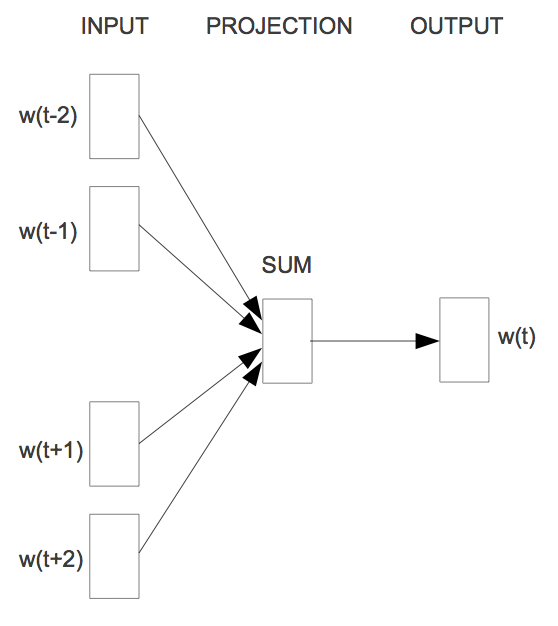
\includegraphics[width=\textwidth]{source//images/posts/cbow.png}\caption{Architecture of CBOW}\label{fig:cbow}\end{figure}

Another different point with traditional models is word2vec using both
pre- and post-contexts of the predicting word. The training complexity
is then

\[
Q = N \times D + D \times \log_2(V)
\]

\subsection{Continuous Skip-gram
Model}\label{continuous-skip-gram-model}

The second model is similar to CBOW, but instead of predicting the
current word based on the context, it tries to maximise classification
of a word based on another word in the same sentence. More precisely, it
uses each current word as an input to a log-linear classifier with
continuous projection layer, and predict words within a certain range
before and after the current word. The architecture is shown in the
following figure (\autoref{fig:skip-gram})

\begin{figure}[h]\centering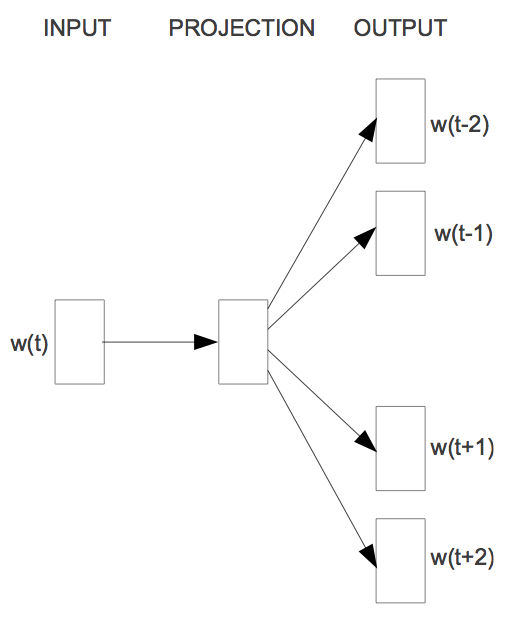
\includegraphics[width=\textwidth]{source//images/posts/skip-gram.png}\caption{Architecture of Skip-gram}\label{fig:skip-gram}\end{figure}

The complexity of Skip-gram model is

\[
Q = 2 \times C \times (D + D \times \log_2(V))
\]

where \(C\) is the maximum distance of the words. Thus, for a particular
\(C\) , for each training word it will select randomly a number
\(R \in [1, C]\), and then use \(R\) words from history and \(R\) words
from the future of the current word as correct labels.

For both CBOW and Skip-gram models, after training, the corresponding
column of the projection matrix is taken out to be the vectors of one
word.

The objective function of Skip-gram models is to maximise the average
log probability

\begin{equation}
\mathcal{O} = \frac{1}{T}\sum_{t=1}^{T} \sum_{-c \leq j \leq c, j \neq 0} \log p(w_{t+j} \mathop{|} w_t)
\end{equation}

where the probability \(p(w_{t+j} \mathop{|} w_t)\) is defined by
softmax function,

\begin{equation}
p(w_{O} \mathop{|} w_I) = \frac{e^{\mathbf{v}^{'\top}_{w_O} \mathbf{v}_{w_I}}}{\sum_{w=1}^V e^{\mathbf{v}^{'\top}_w \mathbf{v}_{w_I}}}
\end{equation}

where \(\mathbf{v}_w\) and \(\mathbf{v}'_w\) are the ``input'' and
``output'' vector representation of \(w\), which are the corresponding
column of projection matrix and the weight matrix between projection and
output layer.

After above work, \cite{mikolov2013distributed} proposed some method to
further speedup the training, such as hierarchical softmax and negative
sampling, and then extended words to phrases. We won't go deep into
these in this post.

\section{Paragraph to Vector}\label{paragraph-to-vector}

Inspired by word2vec, \cite{le2014distributed} extends it to transform a
variable-length of text to a \emph{paragraph vector}. The architecture
is similar with CBOW, as shown in the following figure
(\autoref{fig:paragraph-vec}), except that the additional paragraph
token in input layer, which is mapped to a vector via matrix \(D\).

\begin{figure}[h]\centering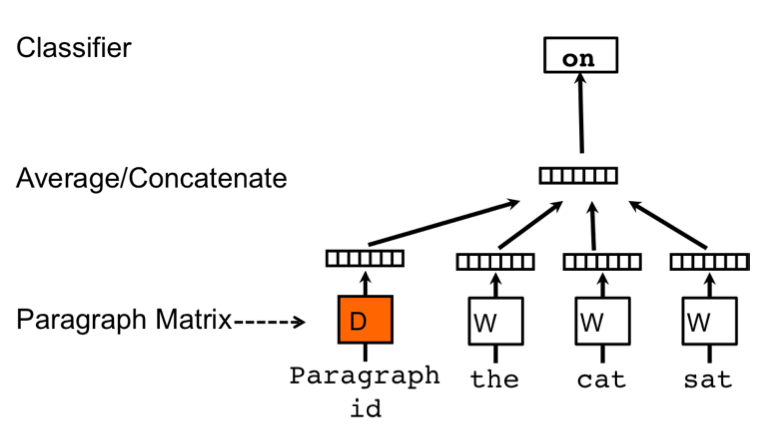
\includegraphics[width=\textwidth]{source//images/posts/paragraph-vec.png}\caption{Architecture of Paragraph Vector}\label{fig:paragraph-vec}\end{figure}

The paragraph token can be thought of as another word. It acts as a
memory that remembers what is missing from the current context -- or the
topic of the paragraph. The contexts are fixed-length and sampled from a
sliding window over the paragraph. The paragraph vector is shared across
all contexts generated from the same paragraph but not across
paragraphs. The word vector matrix \(W\), how-ever, is shared across
paragraphs. At every step of stochastic gradient descent, one can sample
a fixed-length context from a random paragraph, then use them to train
the network. At prediction time, one needs to perform an inference step
to compute the paragraph vector for a new paragraph. This is also
obtained by gradient descent. In this step, one can add one column in
\(D\) and gradient descending on \(D\) while holding \(W\) fixed.

After being trained, the paragraph vectors can also be used as features
for the paragraph and be feed directly to other classifiers.

The most important advantages of paragraph vectors is that they are
learned from unlabelled data. Besides, paragraph vectors also address
some of the key weaknesses of bag-of-words models. First, they inherit
an important property of the word vectors: the semantics of the words.
The second advantage of the paragraph vectors is that they take into
consideration the word order, at least in a small context.

\section{Graph to Vector}\label{graph-to-vector}

\cite{tang2015line} further extends the embedding idea to general
information networks, more specifically, it transfer the vertices in a
graph to vectors.

The goal is to use a low-dimensional vector to represent a vertex in the
graph, while preserving both local and global structure informations. To
derive the model, they first formally defined the local and global
similarity of vertices,

The local similarity is defined by \textbf{First-order Proximity}, which
is the weight \(w_{uv}\) on the edge that connected vertex \(u\) and
vertex \(v\).

The \textbf{Second-oder Proximity} of a pair \((u, v)\) is the
similarity between their neighbourhood network structure.
Mathematically, let \(\mathbf{p_u} = (w_{u,1},...,w_{u,|V|})\) denotes
the first-order proximity of \(u\) with all the other vertices, then the
second-order proximity between \(u\) and \(v\) is determined by the
similarity between \(\mathbf{p_u}\) and \(\mathbf{p_v}\). The
second-order proximity assumes that vertices sharing many connections to
other vertices are similar to each other.

Thus, the graph embedding problem becomes that to convert a vertex to
vector, preserving the first- and second-order proximities.

Their model is called \emph{Large-scale Information Network
Embedding(LINE)}. A graph is denotes by \(G = (V, E)\), where \(V\) is
the set of vertices and \(E\) is the set of edges.

\subsection{LINE with First-order
Proximity}\label{line-with-first-order-proximity}

To model the first-order proximity, for each undirected edge \((i, j)\),
define the joint probability between vertex \(v_i\) and \(v_j\) as

\begin{equation}
p_1(v_i, v_j) = \frac{1}{1 + e^{- \mathbf{u}_i^{\top} \mathbf{u}_j}}
\end{equation}

where \(\mathbf{u}_i \in \mathbb{R}^d\) is the \(d\)-dimensional vector
of vertex \(v_i\).

Note that the empirical probability of \(p_1(\cdot, \cdot)\) can be
defined as

\begin{equation}
\hat{p}_1(v_i, v_j) = \frac{w_{ij}}{\sum_{(i,j) \in E} w_{ij}}
\end{equation}

Thus the objective function of first-order proximity, is to minimise the
following function

\begin{equation}
\mathcal{O}_1 = d(\hat{p}_1(\cdot, \cdot), p_1(\cdot, \cdot))
\end{equation}

where \(d(\cdot, \cdot)\) is the distance between two distributions.
Replacing it with the KL-divergence and omitting some
constants\footnote{The relationship between cross entropy and KL
  distance is \(H(\hat{p}, p) = H(\hat{p}) + D_{KL}(\hat{p}\\|p)\). For
  the purpose of optimising the objective, \(H(\hat{p})\) is constant,
  thus the objective is same as cross entropy.},

\begin{equation}
\mathcal{O}_1 = - \sum_{(i,j) \in E} w_{ij}\log p_1(v_i, v_j)
\end{equation}

Note that the first-order proximity is only applicable for undirected
graphs, not for directed ones.

\subsection{LINE with Second-order
Proximity}\label{line-with-second-order-proximity}

The second-order proximity is applicable for both directed and
undirected graphs. Given a network, without loss of generality, we
assume it is directed.

Each vertex can be treated as a specific ``context'' and vertices with
similar distributions over the ``contexts'' are assumed to be similar.
Therefore, each vertex plays two roles: the vertex itself and a specific
``context'' of other vertices.

Let \(\mathbf{u}_i\) be the representation of \(v_i\) when it is treated
as a vertex, while \(\mathbf{u}'_i\) is the representation of \(v_i\)
when it is treated as a specific ``context''. For each directed edge
\((i, j)\), first define the probability of ``context'' \(v_j\)
generated by vertex \(v_i\) as

\begin{equation}
p_2(v_j \mathop{|} v_i) = \frac{e^{\mathbf{u}_j^{'\top} \mathbf{u}_i}}{\sum_{k=1}^{|V|} e^{\mathbf{u}_k^{'\top} \mathbf{u}_i}}
\end{equation}

where \(|V|\) is the number of vertices or ``contexts''.

And the empirical probability is

\begin{equation}
\hat{p}_2(v_j \mathop{|} v_i) = \frac{w_{ij}}{d_i}
\end{equation}

where \(d_i\) is the out-degree of vertex \(i\), i.e.
\(d_i = \sum_{k \in N(i)} w_{ik}\), where \(N(i)\) is the set of
out-neighbours of \(v_i\).

Similarly, the objective of second-order proximity is

\begin{equation}
\mathcal{O}_2 = \sum_{i \in V}\lambda_i d(\hat{p}_2(\cdot \mathop{|} v_i), p_2(\cdot \mathop{|} v_i))
\end{equation}

For simplicity, set \(\lambda_i = d_i\), then replacing
\(d(\cdot, \cdot)\) with the KL-divergence and omitting some constants,

\begin{equation}
\mathcal{O}_2 = - \sum_{(i,j) \in E} w_{ij}\log p_2(v_j \mathop{|} v_i)
\end{equation}

\bibliographystyle{unsrt}

\bibliography{source/assets/printables/references}

\end{document}
